\documentclass[11pt, a4paper]{article} %draft

\usepackage{graphicx,color}
\usepackage{amssymb, amsmath, array}
\usepackage[english]{babel}
\usepackage[babel=true]{csquotes}
\usepackage{verbatim}
\usepackage{float}
\usepackage{caption}
\usepackage{subcaption}
\usepackage{url}

\begin{document}

% Example of title page for the projects carried out within DEDIS
% Copied from lasec

% Simply include it in your mastex tex file:
%        % Example of title page for the projects carried out within DEDIS
% Copied from lasec

% Simply include it in your mastex tex file:
%        % Example of title page for the projects carried out within DEDIS
% Copied from lasec

% Simply include it in your mastex tex file:
%        \input{cover}


% Updated October 2016


\newcommand{\logoepfl}[0]{
  \begin{center}
    
\includegraphics[width=6cm]{logo_epfl_coul.eps}
  \end{center}
  \vspace{0.3cm}
  \hrule
}
\newcommand{\project}[1]{
  \begin{center}
    \large{#1}
  \end{center}
  \vspace{1cm}
}
\newcommand{\department}[1]{
  \begin{center}
    \large{#1}
  \end{center}
}
\newcommand{\lab}[1]{
  \begin{center}
    \large{#1}
  \end{center}
}
\newcommand{\supervisor}[3]{
  \begin{center}
    \begin{normalsize}{
        \bf #1}\\#2\\#3
    \end{normalsize}
  \end{center}
}
\renewcommand{\author}[1]{
  \begin{center}
    \Large{#1}
  \end{center}
  \vspace{0.5cm}
}
\renewcommand{\title}[1]{
  \vspace{3cm}
  \begin{center}
    \huge{#1}
  \end{center}
  \vspace{1.7cm}
}
\renewcommand{\date}[2]{
  \begin{center}
    \normalsize{#1 #2}
  \end{center}
  \vspace{0.5cm}
}


\thispagestyle{empty}


% begin title page
  \logoepfl

  \title{BLS cosigning via gossip protocol~--- DRAFT}

  \author{Lukas Gelbmann}
  \department{School of Computer and Communication Sciences}
  \lab{Decentralized and Distributed Systems lab}
  \project{Semester Project}

  \date{June}{2019}

  \begin{center}
    \begin{tabular}{cc}
      \begin{tabular}{p{4.0cm}}
        \supervisor{Responsible}{Prof. Bryan Ford}{EPFL / DEDIS}
      \end{tabular}&
      \begin{tabular}{p{4.0cm}}
        \supervisor{Supervisor}{Cristina Basescu}{EPFL / DEDIS}
        \supervisor{Supervisor}{Gaylor Bosson}{EPFL / DEDIS}
      \end{tabular}
    \end{tabular}
  \end{center}

% end title page



% Updated October 2016


\newcommand{\logoepfl}[0]{
  \begin{center}
    
\includegraphics[width=6cm]{logo_epfl_coul.eps}
  \end{center}
  \vspace{0.3cm}
  \hrule
}
\newcommand{\project}[1]{
  \begin{center}
    \large{#1}
  \end{center}
  \vspace{1cm}
}
\newcommand{\department}[1]{
  \begin{center}
    \large{#1}
  \end{center}
}
\newcommand{\lab}[1]{
  \begin{center}
    \large{#1}
  \end{center}
}
\newcommand{\supervisor}[3]{
  \begin{center}
    \begin{normalsize}{
        \bf #1}\\#2\\#3
    \end{normalsize}
  \end{center}
}
\renewcommand{\author}[1]{
  \begin{center}
    \Large{#1}
  \end{center}
  \vspace{0.5cm}
}
\renewcommand{\title}[1]{
  \vspace{3cm}
  \begin{center}
    \huge{#1}
  \end{center}
  \vspace{1.7cm}
}
\renewcommand{\date}[2]{
  \begin{center}
    \normalsize{#1 #2}
  \end{center}
  \vspace{0.5cm}
}


\thispagestyle{empty}


% begin title page
  \logoepfl

  \title{BLS cosigning via gossip protocol~--- DRAFT}

  \author{Lukas Gelbmann}
  \department{School of Computer and Communication Sciences}
  \lab{Decentralized and Distributed Systems lab}
  \project{Semester Project}

  \date{June}{2019}

  \begin{center}
    \begin{tabular}{cc}
      \begin{tabular}{p{4.0cm}}
        \supervisor{Responsible}{Prof. Bryan Ford}{EPFL / DEDIS}
      \end{tabular}&
      \begin{tabular}{p{4.0cm}}
        \supervisor{Supervisor}{Cristina Basescu}{EPFL / DEDIS}
        \supervisor{Supervisor}{Gaylor Bosson}{EPFL / DEDIS}
      \end{tabular}
    \end{tabular}
  \end{center}

% end title page



% Updated October 2016


\newcommand{\logoepfl}[0]{
  \begin{center}
    
\includegraphics[width=6cm]{logo_epfl_coul.eps}
  \end{center}
  \vspace{0.3cm}
  \hrule
}
\newcommand{\project}[1]{
  \begin{center}
    \large{#1}
  \end{center}
  \vspace{1cm}
}
\newcommand{\department}[1]{
  \begin{center}
    \large{#1}
  \end{center}
}
\newcommand{\lab}[1]{
  \begin{center}
    \large{#1}
  \end{center}
}
\newcommand{\supervisor}[3]{
  \begin{center}
    \begin{normalsize}{
        \bf #1}\\#2\\#3
    \end{normalsize}
  \end{center}
}
\renewcommand{\author}[1]{
  \begin{center}
    \Large{#1}
  \end{center}
  \vspace{0.5cm}
}
\renewcommand{\title}[1]{
  \vspace{3cm}
  \begin{center}
    \huge{#1}
  \end{center}
  \vspace{1.7cm}
}
\renewcommand{\date}[2]{
  \begin{center}
    \normalsize{#1 #2}
  \end{center}
  \vspace{0.5cm}
}


\thispagestyle{empty}


% begin title page
  \logoepfl

  \title{BLS cosigning via gossip protocol~--- DRAFT}

  \author{Lukas Gelbmann}
  \department{School of Computer and Communication Sciences}
  \lab{Decentralized and Distributed Systems lab}
  \project{Semester Project}

  \date{June}{2019}

  \begin{center}
    \begin{tabular}{cc}
      \begin{tabular}{p{4.0cm}}
        \supervisor{Responsible}{Prof. Bryan Ford}{EPFL / DEDIS}
      \end{tabular}&
      \begin{tabular}{p{4.0cm}}
        \supervisor{Supervisor}{Cristina Basescu}{EPFL / DEDIS}
        \supervisor{Supervisor}{Gaylor Bosson}{EPFL / DEDIS}
      \end{tabular}
    \end{tabular}
  \end{center}

% end title page


\newpage
\pagenumbering{roman}
\begin{abstract}
Decentralized cosigning protocols have the main purpose of collecting digital signatures of a message from many peers. This type of protocols is used in two existing implementations. The first one is BLS CoSi which uses trees to get the signatures and aggregate them, the second one is a gossip protocol.

This semester project develops and compares alternative implementations of the gossip-based aggregation. The main goal of the new implementations is to reduce the bandwidth used and to be relatively fast. 

Furthermore, this project adds an hybrid implementation of trees and gossiping inside Cothority's ONet library, which is used for a new implementation of signature aggregation. Finally, there is an analysis of this protocol, measuring its performance and finding possible future improvements.
\end{abstract}
\tableofcontents



\newpage

\pagenumbering{arabic}
% Start page count
\setcounter{page}{1}

\section{Introduction}

Decentralized cosigning protocols collect signatures of a message, these signatures come from a group of many distributed peers. The collected signatures are then aggregated and 
\emph{cosigning} (collective signing) protocols are used to validate the message.
This type of protocol has many uses, for example a network authority (e.g. a certificate authority) can release an statement and have it validated by many other witnesses to improve security. This could prevent a malicious third party to abuse stolen private keys of the authority ~\cite{Syta16}.
Another example is software updates signatures, which can have the added security of many witnesses for software builds~\cite{Niki17}, and protect users from updates that introduce backdoors or malware that could be provided by a compromised update server, or even by law enforcement intrusion~\cite{Ford16}.

The \emph{\mbox{ByzCoin}} protocol~\cite{Koko16} developed at the DEDIS~lab at EPFL uses a cosigning protocol as the core of its blockchain and cryptocurrency implementation.
In \mbox{ByzCoin}, a proposed block has to be signed by a minimum threshold number of nodes to be accepted as part of the blockchain. Using the cosigning protocol allows faster transaction confirmations, since blocks that contain transactions are appended to the blockchain much faster. Therefore message confirmation latency is very low, and this is one of the main improvements of \mbox{ByzCoin} over other cryptocurrencies such as Bitcoin. For fault tolerance, the cosigning protocol must tolerate a certain number of offline or malicious nodes. No single node should process an overwhelming amount of messages in order for the protocol to scale well, and the size of messages should be kept low.

The goal of this semester project is to implement and evaluate alternative gossip protocol models for cosigning messages, and also a protocol in \emph{ONet} (The Cothority Overlay Network Library) to use for building collective signatures.
An existing cosigning protocol built at the DEDIS~lab, \emph{BLS~CoSi}~\cite{Blscosi} is used as the reference for performance comparison. Another existing gossip-based cosigning protocol~\cite{ProjExisting} is also used as a starting point for the implementation.
BLS~CoSi uses the Boneh-Lynn-Shacham signature scheme~\cite{Boneh01}, which supports \emph{multi-signatures}~\cite{Boneh03}.
Multi-signatures are short signatures that can be used to verify the signing of a common message by a large number of parties.

All cosigning protocols, existing and new, use a multi-signature scheme based on BLS signatures to reduce the amount of data transferred and stored, this type of signatures are relatively recent and proposed by Boneh, Drijvers and Neven~\cite{Boneh18}.
The existing BLS~CoSi implementation is not efficient when some of the nodes fail, and the existing Gossip-based cosigning protocol fixes this problem, but has a increase of bandwidth and propagation time, so there is plenty of room for improvement. A gossip protocol is well-suited for the task of improving fault tolerance, but has some downsides that will be analyzed.
This report introduces new cosigning protocols and then analyzes them based on an experimental evaluation using Cothority simulations.

The main goal of the new protocols is to improve the efficiency when compared to the existing BLS~CoSi and gossip-based protocol. The protocol should be fast, while avoiding overwhelming participating nodes and being fault tolerant.
The new protocol is designed mainly for the use case of \mbox{ByzCoin}, although other applications are certainly possible.

Section 2 of this report gives some background on gossip protocols and the cryptographic tools used both in the old and new cosigning protocols, and outlining how the old protocols work.
Section 3 presents the new gossip protocols' design and implementation.
In Section 4, the evaluation methodology and setup used in the simulations is shown. Plots of the results are included.
Finally, Section 5 is the conclusion, which discusses the findings, mentions the limitations, gives some insight on future work and improvements, and closes the report.



\section{Background}

\subsection{Gossip protocols}
\label{gossip}

Gossip protocols are often used for information dissemination and computing an aggregate between many nodes~\cite{Birm07}. Generally, they can be used for a range of tasks where information needs to be shared between different nodes.
They provide many useful properties while maintaining reasonable efficiency.
One important such property is logarithmic \emph{mixing time}: if the number of nodes is $n$, a correctly designed gossip protocol propagates a new piece of information to all peers in $O(log(n))$ time, assuming nodes are not overwhelmed by the rate of information transfer~\cite{Birm07}.
In addition to this, the number of messages that a single node sends and receives is constant among the existing peers. Another advantage is the simplicity of gossip protocols: all participating nodes will usually run the same code.

A typical basic gossip protocol repeatedly runs three steps in a loop: \emph{peer selection}, \emph{data exchange} and \emph{data processing}~\cite{Kerm07}.
The first step consists of peer selection, here the node chooses one or more peers to exchange information with, typically this selection is random. Choosing a new set of random peers on every gossip round is a simple and effective way to achieve fault tolerance.
In the second step, data exchange, data is sent to or received from the peers according to the selection made in the previous step. There are two types of data exchange models, \emph{push} and \emph{pull}. The \emph{push model} sends information to the peer and no reply is expected. In the \emph{pull model}, a request is sent, to which the peer responds with the information they know. Is is also possible to combine both of the models in one protocol.
The third step in the gossip protocol is data processing, this step is optional. Here the new information is processed or passed to a higher application layer. Type of processing and how it is done depends on the domain and application of the protocol.

A gossip protocol that is concerned with information dissemination can be analyzed by looking at the different states in which a node can find itself in regards to an update~\cite{Jela13}.
In this context, an update is a piece of information that is being spread. There are usually up to three states called \emph{susceptible~(S)}, which means the node does not know about the update, \emph{infected~(I)}, meaning the node is actively spreading the update, and \emph{removed~(R)}, which means that the node knows about the update, but is no longer actively spreading it.
Using these definitions, some gossip protocols use a SI~model, where a node starts in state~S and switches to state~I when it learns about an update, after which it can no longer change its state with regards to this update. Another possible model is the SIR~model, where a change to state~R can happen after the node transitions to state~I.

\subsection{Multi-signatures}

A \emph{digital signature} is a tool of asymmetric cryptography (also called public-key cryptography), which is computed from a message and a private key, and can be verified using the corresponding public key and the message.
\emph{Cosigning} or collective signing, as used in this project and report, means that multiple nodes digitally sign the same message or statement.
For this purpose, a \emph{multi-signature} can be used. This is a compact value that proves that multiple nodes have signed the same message~\cite{Boneh18}. A multi-signature is computed by aggregating many signatures from different nodes.
The advantage of assigning a multi-signature to the message, instead of a list of the signatures from different nodes, is that a multi-signature is smaller. This is especially important in protocols where many cosignatures are exchanged between nodes, as is the case in ByzCoin~\cite{Koko16} (a decentralized cryptocurrency using a Byzantine consensus protocol).

The multi-signature scheme used in the new protocol is based on work by Boneh, Drijvers and Neven~\cite{Boneh18} and is implemented under the name \emph{BDN} in the cryptographic library \emph{Kyber}~\cite{Kyber}.
BDN multi-signatures are based on the Boneh-Lynn-Shacham (\emph{BLS}) signature scheme~\cite{Boneh01} and use commutative groups of prime order both for the signatures and the public keys.
In the version of the BDN scheme that is used in the existing cosigning protocol and that will also be used in the new protocols implemented, the public keys of all nodes have to be known in advance, even if not all of them end up signing the message.
The public keys are collectively used to create a unique integer coefficient for each signatory: $\alpha_1$ for the first node, $\alpha_2$ for the second, and so on.
In a set of three nodes signing the same message, where $S_i$ is the signature of node~$i$, the multi-signature~$S$ is then computed as $S = \alpha_1 * S_1 + \alpha_2 * S_2 + \alpha_3 * S_3$ (using additive group notation).
A multi-signature from just part of the nodes, such as $\alpha_1 * S_1 + \alpha_3 * S_3$, is equally possible.
Thanks to the associative and commutative properties (order of operands and grouping of operands does not alter the result), partial multi-signatures from two or more disjoint sets of peers can be added to form a new valid multi-signature. A more in-depth explanation of BDN is found in the paper presenting the scheme~\cite{Boneh18}, and BLS is explained in a relevant article by Snigirev~\cite{Snig18}.

To verify a multi-signature the verifier must know the public keys of all the nodes that are part of the group, including those who did not end up signing. In the context of the cosigning protocols relevant to this project, this is not a problem, since all nodes know the public keys of all peers.
The verifier must also know which nodes contributed to a multi-signature, so it uses the corresponding public keys for the verification process. This is solved by storing a bitmap together with each multi-signature that indicates the contributing nodes.


\subsection{Existing protocol implementations}

\subsubsection{BLS~CoSi protocol}

In BLS~CoSi~\cite{Blscosi}, a protocol instance is initiated when a cosignature is requested on some node by a client from a higher application layer.
BLS~CoSi is a part of the \emph{Cothority} framework~\cite{Coth}, which handles authenticated communication between nodes, and also is in charge of the distribution of public keys and membership of nodes.
Therefore, it can be assumed that all nodes know all public keys from the start and that the set of peers is known and constant for the duration of the protocol. Generally, there is a certain threshold of nodes that must sign a message it before it is considered a valid cosignature.
For this project and report, we assume that \emph{Byzantine consensus} is needed, which requires the assumption that up to $f$ out of $n = 3f+1$ nodes may be faulty (this includes both offline and malicious nodes) and we require $2f+1$ nodes, i.e.~just above two thirds of nodes, to sign a message~\cite{Koko16}.

BLS~CoSi works by arranging all participating nodes in a tree of depth~3.
The root of this tree is the node where the protocol instance is initiated, which is simultaneously the node where the cosignature needs to be returned to an application layer in the end.
An initial signature request containing the message to be signed is sent by the root to all its child nodes in the tree.

These internal nodes then send a signature request to their children, which are leaf nodes. The leaf nodes reply by sending their signature to their parent nodes, who then aggregate the received signatures.
They add their own signature and return the aggregated signature to the root, who then combines the aggregates and its own signature to form the final cosignature. Each node can also choose not to sign the message, and in that case, instead of a signature, it sends a refusal message.

One problem of BLS~CoSi is that if a child of the root is faulty and does not return the expected aggregate, the root potentially misses out on a lot of signatures.
To mitigate this problem, the root rearranges the tree and tries again if, for example, it has not heard back from a child after a few seconds.
However, this solution is not ideal, as it is possible that multiple attempts are needed, which can cost a lot of time and bandwidth.

\subsubsection{Gossip aggregation protocol}

As the result of a previous project \cite{ProjExisting}, there is an implementation of message cosigning that uses a gossip protocol. The interface for calling this protocol is the same as for BLS CoSi. As before, the protocol starts with a single node, the root, needing a cosignature. Any node can start a protocol instance and will then be the root for this instance. The root has a special role in the protocol, as the root needs to return a cosignature to an application layer in the end.

During the main part of the protocol, only one type of message is exchanged between nodes, called a \emph{rumor message}. It contains the statement to be signed as well as all the signatures the sender has seen so far.
At the moment the protocol starts, only the root knows about the protocol.
The other nodes start participating after they receive a rumor message for the first time.

The behavior of each node during this initial phase of the protocol is simple.
After receiving a rumor message for the first time, the node adds its own signature to its collection of known signatures (assuming that the node chooses to sign the statement).
A node also adds all signatures to its collection when they are received for the first time.
Each node periodically sends a rumor message, containing the full collection of known signatures, to a set of $r$ different randomly selected peers ($r$ is smaller than the number of nodes~$n$).
This sending of rumor messages happens at a regular interval~$t$, typically a fraction of a second in a context like ByzCoin.
The parameters $r$ and~$t$ have the same fixed value for all nodes.

This implementation also has two variations on how the aggregation is done. The first and the more simple one, aggregates signatures at the root node after enough signatures from peers have been received. The second variation, aggregates signatures earlier along a conceptual binary tree.
Each leaf in this tree stands for a signature from a single signatory.
All other nodes in the binary tree stand for the aggregation of their children.
For example, with four potential signatories $A$, $B$, $C$ and~$D$, there are four leaves, one for each of them.
One level up, we might have one parent for the aggregation $\{A, B\}$ and one for $\{C, D\}$.
At the top of the binary tree is the aggregation of these two: $\{A, B, C, D\}$.
The second protocol variant aggregates signatures if and only if the aggregation exists in this binary tree.
This way, there are never any two multi-signatures from disjoint sets of signatories.

As soon as the root node has received a threshold number of signatures through this process of gossip, it sends an aggregated cosignature to the application that requested it.
At this point, the protocol has fulfilled its task, and all that is left to be done is to wind down the protocol.
This needs to be done with some care; after all, the other nodes do not know when the protocol is done.
To signal that the protocol is finished, the root sends a \emph{shutdown message} to $s$ different randomly selected peers and enters \emph{shutdown mode}, where $s$ is another parameter with the same fixed value for all nodes.
In shutdown mode, incoming rumors are answered with a shutdown message and incoming shutdown messages are ignored.
The stored collection of signatures is no longer needed in shutdown mode.
When a node receives a valid shutdown message, it sends the message on to $s$ different randomly selected peers and enters shutdown mode.

The rumor messages act as \emph{push} messages most of the time.
However, when they reach a node in shutdown mode, they act more like a \emph{pull} message, pulling the shutdown message. The protocol is designed to spread information quickly, with efficiency only being a secondary concern. This is why entering shutdown mode is only possible after it has been proven that the root has received a valid cosignature.

This implementation is more efficient in a scenario with failing nodes than the BLS~Cosi protocol, but at the cost of a higher protocol duration, and increased bandwidth use. It will be used as a benchmark for alternative implementations of gossip-based aggregation by trying variants of the gossip model used.

\subsection{Cothority Overlay Network Library - ONet}

The Overlay-Network (ONet) is a library for simulation and deployment of decentralized, distributed protocols. For this purpose, it offers a framework for research, simulation, and deployment of crypto-related protocols; with a special emphasis on decentralized, distributed protocols. It is used in research for testing out new protocols and running simulations, as well as in production to deploy those protocols as a service in a distributed manner.

ONet is developed by DEDIS/EFPL as part of the Cothority project that aims to deploy a large number of nodes for distributed signing and related projects. In cothority, nodes are commonly named \emph{conodes}. A collective authority or \emph{cothority} is a set of conodes that work together to handle a distributed, decentralized task. ONet offers an abstraction for tree-based communications between thousands of conodes.

ONet allows you to set up protocols, services and apps.
Protocols are a short-lived set of messages being passed back and forth between one or more conodes,
Services define an API usable by client programs and instantiate protocols, and apps communicate with the service-API of one or more conodes \cite{ONet}.

\section{Design and implementation}

\subsection{Alternative gossip-based aggregation protocols}

Similar to the existing BLS~CoSi and Gossip with aggregation implementations, the new cosigning protocol is written in Go and fits into the Cothority project~\cite{Coth}.
It makes use of different tools developed by the DEDIS lab, including Kyber~\cite{Kyber}.

The interface for calling the new protocol is the same as for BLS~CoSi.
As before, the protocol starts with a single node, which is called the \emph{root}, requesting a cosignature.
Any node can start a protocol instance and will then be the root for this instance.
The root has a special role in the protocol, as the root needs to return a cosignature to an application layer in the end.


The parameters $r$ (number of randomly selected nodes for each gossip round), $s$ (number of randomly selected nodes for shutdown message propagation) and $t$ (time interval between gossiping rounds) are sent along with rumor messages in our current implementation to help us test the effects of these parameters in experiments.
In a real-world implementation, they would be fixed in advance.

For this part of the project, the following alternative gossip protocol models were implemented.

\subsubsection{Mask protocol}

The most important change for this gossip implementation when compared to the existing aggregation gossip one is the use of both push and pull messages. This is achieved by adding a bitmap mask of all the signatures known by the node who is sending the message, so the receiving node can compare this mask with the signatures it has already seen, and then send a pull message to request the specific signatures they still need. In theory this will increase the number of messages sent by nodes, but could potentially reduce the total bandwidth used, since we are reducing the impact of a failing node when compared to the previous tree based implementations. It should also reduce the propagation time needed, since nodes will be able to ask for the signatures they need, and they can be sent not only by the signing peer, but any peer who has seen this signature.

During the main part of the protocol, only one type of message is exchanged between nodes, called a \emph{rumor message}.
It contains the statement to be signed, the sender's  signature, and a bitmap of all the signatures the node knows and are available for requests. 

Similar to the previous gossip protocol, after receiving a rumor message for the first time, the node adds its own signature to its collection of known signatures (assuming that the node chooses to sign the statement).
A node also adds all signatures to its collection when they are received for the first time.
Each node periodically sends a rumor message (with the mentioned contents), to a set of $r$ different randomly selected peers ($r$ is smaller than the number of nodes~$n$).
This sending of rumor messages happens at a regular interval~$t$. These parameters $r$ and~$t$ have the same fixed value for all nodes.

As soon as the root node has received a threshold number of signatures through this process of gossip, it sends an aggregated cosignature to the application that requested it.
At this point, the protocol has fulfilled its task, and for the final shutdown step, the root sends a \emph{shutdown message} to $s$ different randomly selected peers and enters \emph{shutdown mode}, where $s$ is another parameter with the same fixed value for all nodes.
In shutdown mode, incoming rumors are answered with a shutdown message and incoming shutdown messages are ignored. When a node receives a valid shutdown message, it sends the message on to $s$ different randomly selected peers and enters shutdown mode. To prevent an attack where a malicious node causes other nodes to enter shutdown mode prematurely, shutdown messages have to be signed by the root.
Invalid messages are simply ignored.


\subsubsection{Mask aggregation protocol}

For this variation on the mask protocol explained in the previous paragraphs, we also use both push and pull message and a bitmap mask of the signatures known. The difference is in the signature being sent, which instead of being a single one, is a multi-signature, the aggregation of all the signatures known by the sender. The receiving node will store this aggregated signature, see if it comes from a disjoint set of signatories when compared to the signatures it knows. If the received multi-signature does not conflict with the signatures known by the receiver, it will aggregate them. If it does conflict, it will be compared with other received and stored multi-signatures, aggregated if possible and stored.
All signatures and multi-signatures received are combined in all the possible aggregations, until a node creates a multi-signature with enough signatures to satisfy the protocol.

After the aggregation and storing of multi-signatures, if it doesn't have enough signatures yet, the node will compare the received bitmap mask with the signatures it has already seen, and send a pull message to request the combination of signatures they are missing. In theory this will increase the number of messages sent by nodes, but could potentially reduce the total bandwith used, since we are reducing the impact of a failing node when compared to the previous tree based implementations. It should also reduce the propagation time needed, since nodes will be able to ask for the signatures and/or multi-signatures they need, and they can be sent not only by the signing peer, but any peer who has seen this signature.

The rumor message for this version of the protocol contains the statement to be signed, the sender's  multi-signature, and a bitmap of all the signatures the node knows and are available for requests. 

Similar to the previous gossip protocol, after receiving a rumor message for the first time, the node adds its own signature to its collection of known signatures (assuming that the node chooses to sign the statement).
A node also adds all signatures and multi-signatures to its collection when they are received for the first time.
Each node periodically sends a rumor message, to a set of $r$ different randomly selected peers ($r$ is smaller than the number of nodes~$n$). This happens at a regular interval~$t$, and both $r$ and~$t$ have the same fixed value for all nodes.

As soon as the root node has received a threshold number of signatures through this process of gossip, it sends an aggregated cosignature to the application that requested it, shutdown messages are propagated, and then the protocol is finished.


\subsubsection{Aggregation protocol with homomorphic subtraction}

In this variation of the gossip protocol, both push and pull messages are sent. The rumor message contains the statement to be signed, the sender's multi-signature, and a bitmap mask of the signatures known by the sender. On the receiving end, the peer will try to aggregate the multi-signature received with its own multi-signature. Any overlapping signatures are subtracted using the scalar point homomorphic subtraction in the Kyber library~\cite{Kyber}, so the result of this subtraction can be aggregated with the received multi-signature. If for the subtraction operation the node needs some specific signatures that they don't know, they will reply with a pull message to the sender. This will only be done if the needed signature is available according to the bitmap mask they received in the message. 

Each node periodically sends a rumor message, to a set of $r$ different randomly selected peers, at a regular interval~$t$, until the signature minimum threshold is reached, then the protocol is shutdown and completed with the delivery of the aggregated cosignature to the application to requested it from the root node.

Because of time constraints, this implementation couldn't be completed, so the evaluation chapter of this report doesn't contain results for this implementation.

\subsection{Hybrid protocol in ONet}

For the implementation of cosigning in the Cothority Overlay Network Library, the first design tried to insert the gossip logic into the treenode layer of ONet, since this layer had access to the TreeNodeInstance class, which represents a Cothority protocol instance, which is the main type of protocol that would use this library. Here we identified a problem with trying to add the gossip protocol in the ONet library. The shutdown of the gossiping would be problematic, since it requires a shutdown message to be propagated to enough peers, and this would affect all the metrics we are using to measure efficiency (duration time, number of messages sent and bandwith used).
Then we decided that to keep the best of both protocols (tree based propagation and gossip based propagation), we would implement a hybrid of both, having a \emph{sendHybridRumor()} function in the overlay layer of ONet. This function can be used for the implementation of cosigning in a protocol external to ONet that has it as a dependency.

Consequently, the new type of message added to the overlay layer of ONet, would be a hybrid between a rumor message and a tree-based message. For this hybrid-rumor propagation, there are two sub-rounds in every gossiping round. First, we create a $m$-ary tree with a depth of 2. The root node and all intermediary nodes would have a maximum of \emph{m} children nodes, which is a parameter received by the hybrid-rumor function. Then, once this tree is created, for the first sub-round the root sends the rumor to the intermediary nodes. They sign the message, send a response, and forward the rumor received to the leaf nodes.
These leaf nodes just send their response to the intermediary node, which in turn forwards it to the root. After time $t$ (which is also a configurable parameter), the root node checks how many responses it has received. If it has received all the signatures from the tree, it finishes the gossiping round. If it is missing any signatures, the second sub-round starts, here it tries to contact the missing nodes directly, so a failing intermediary node doesn't affect the effectiveness of the propagation as much.

The rumor message is stored in all the instances of overlay of the nodes that have received it. The responses received are stored only in the root node. There is also a static function added in the overlay, that has as input the rumor message that a node received, and the output of this function is sent as the response message. By default this function just returns the same message it received, but it can be customized by a Cothority protocol with its own implementation. This function will allow us to use the hybrid-rumor in a gossip protocol, since the signature of the message can be placed in this place, so the overlay layer doesn't need to know about Kyber suites or signature schemes.

After this was completed inside ONet, we developed a cosigning protocol that simply runs many rounds of Hybrid Rumors being sent, until the threshold of received signatures is met. Finally these signatures are aggregated, the multi-signature is validated and sent to the application that requested the cosigning.

\section{Evaluation and results}
\label{evares}

\subsection{Methodology used for experimentally evaluating the protocol}

To evaluate the new gossip protocols, they were tested in Cothority simulations and compared to the previous implementation under varying conditions.
These conditions include the number of nodes, the number of failing nodes, and an artificial message delay, which is used to simulate real-world network delays.
The delay for any given message was randomly picked from a uniform distribution between a fixed minimum and maximum delay.
A failing node, in our simulations, drops all incoming messages and sends no messages, effectively causing the node to be offline.
If a node is not failing, it is considered \emph{active} and functions correctly, the root was active in all simulations.
All experiments were run on a single machine with six 2.20~GHz Intel Core~i7 processors under Ubuntu~18.04.

Three metrics were used to evaluate the protocols.
The most important metric is the time it takes until the root returns the cosignature, called the \emph{protocol duration}.
The other two metrics we measured are the number of messages sent per active node and the amount of data sent per active node.
Both rumor messages and shutdown messages (when existing) are included in these metrics.


\subsection{Parameter values used in simulations}
\label{defaults}

The parameters come in two groups: environment parameters that are not within the node's control, and protocol parameters that affect how the nodes behave.

For the environment parameters, we simulated different combinations of total number of nodes and number of failing nodes, as explained in Table 1.

\begin{table}[]
  \caption{Number of nodes used in simulations}
\centering
\begin{tabular}{|c|c|}
\hline
Total number of nodes & Number of Failing nodes   \\ \hline
7                     & 0-2     \\ \hline
16                    & 0-5    \\ \hline
25                    & 0-8    \\ \hline
36                    & 0-11  \\ \hline
\end{tabular}
\end{table}

In addition to this, a small range of possible delays ($0.01$~seconds between the minimum and maximum delay) is specified to prevent unnatural effects where, for example, messages from different nodes always arrive at the same time.

\begin{itemize}
    \item Minimum message delay: $0.095$~seconds
    \item Maximum message delay: $0.105$~seconds
\end{itemize}

The threshold of signatories for a valid cosignature is always set to $n~-~\lfloor \frac{n-1}{3} \rfloor$ because this is the value that is used in ByzCoin.
The default values for the other protocol parameters are as follows.

\begin{itemize}
    \item Number of recipients for each rumor message: $r = 3$
    \item Interval between sending out rumor messages: $t = 0.07$~seconds
    \item Number of initial shutdown-message recipients: $s = 2$
\end{itemize}

These default values for protocol parameters were chosen as a compromise between protocol speed and efficiency.

The evaluation done has two parts, the first one is the comparison between the gossip protocol implementations, to see how the efficiency performance has improved or decreased. The second part compares the ONet Hybrid protocol with the existing gossip protocol, for evaluation of the difference that the implementation approach makes in the performance.

\subsection{Comparison of the gossip protocol implementations}

For the first part, the new gossip protocol was compared to BLS~CoSi with varying numbers of nodes and failing nodes, using the parameters mentioned in the previous paragraphs. The duration of the mask protocol was fairly stable, always measuring below 1.5~seconds in this set of experiments.
With very few failing nodes, it performs similar to the existing implementation, and with a high number of failing nodes, the mask protocol is only slightly slower (around 0.1 seconds).The mask aggregation protocol had a larger protocol duration in all the scenarios.
The timings are shown for $n = 36$ in Figure~\ref{fig1time}. Each box goes from the first quartile to the third quartile. The horizontal line is the median.

\begin{figure}[H]
    \centering
    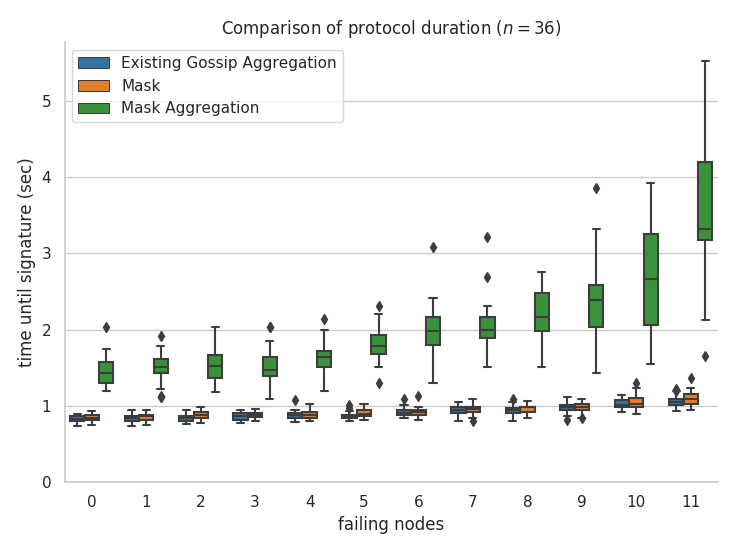
\includegraphics[width=1\textwidth]{images/aggregation_round_wall_sum_36.png}
    \caption{Timings until a cosignature was returned using the different variations of gossip protocol. }
    \label{fig1time}
\end{figure}

For $n = 36$, if we compare the number of messages sent by every node, as seen in Figure~\ref{fig1num}, both mask protocol and mask aggregation protocol send more messages than the existing implementation, since they send pull messages when possible, to get the signatures they need from other peers. Nevertheless, if we compare the amount of data transferred (bandwidth used) by every node, the mask protocol performs slightly better than the existing gossip aggregation, with a consistent improvement of 100kb per node, this can be observed in Figure~\ref{fig1data}. The mask aggregation protocol has a larger amount of bandwidth used, this might be caused by the constant pulling of all the different combination of multi-signatures that are available, so when a node has k signatures, there are $2^{k} - 1$ possible sets of combinations (excluding an empty set), and all of these are propagated by nodes requesting them when they know about them. This explains the increased bandwidth for the mask aggregation implementation.

\begin{figure}[H]
    \centering
    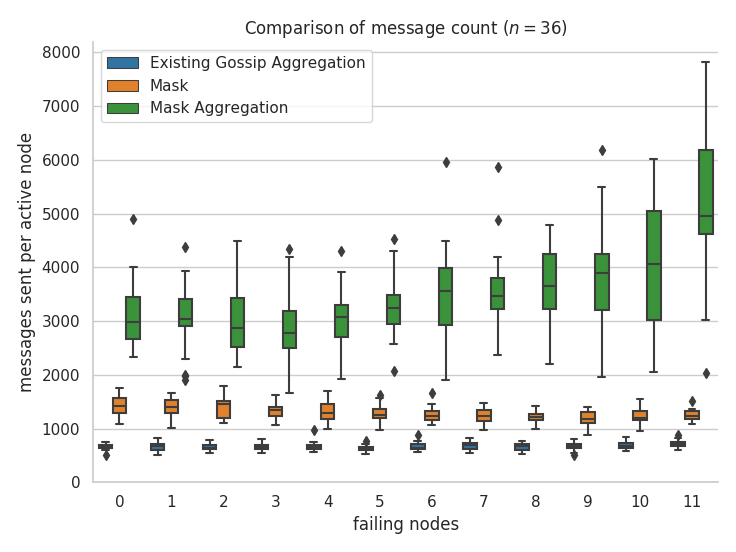
\includegraphics[width=0.91\textwidth]{images/aggregation_bandwidth_msg_tx_sum_36.png}
    \caption{Number of messages sent per active node using different variations of gossip protocol.}
    \label{fig1num}
\end{figure}

\begin{figure}[H]
    \centering
    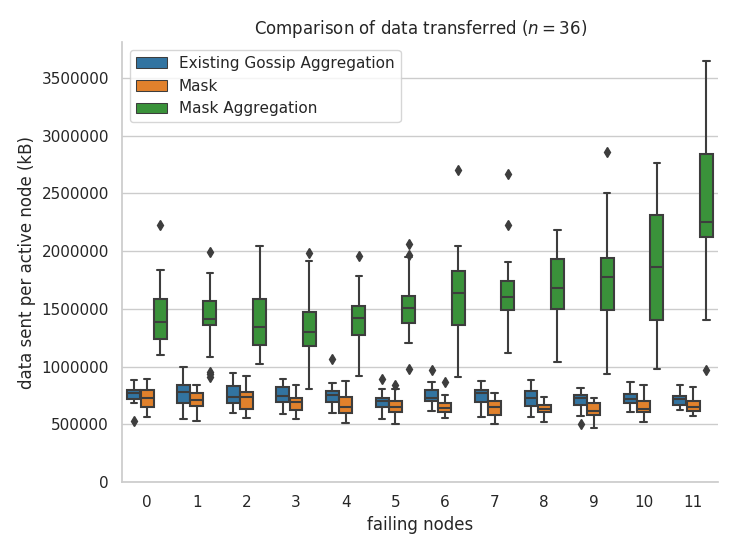
\includegraphics[width=0.91\textwidth]{images/aggregation_bandwidth_tx_sum_36.png}
    \caption{Amounts of data transferred per active node using different variations of gossip protocol.}
    \label{fig1data}
\end{figure}


Other results for simulations with different number of nodes, are available in the form of plots in Appendix~\ref{axresults}.

\subsection{Comparison of the ONet implementation with the existing gossip aggregation}

In the second part, the new ONet hybrid protocol is compared to the existing gossip protocol implementation with the same parameters mentioned earlier.
We can observe that the performance is improved in all the metrics, the number of messages and bandwidth used is decreased significantly, and the protocol duration also has a considerable improvement.
Here we can see the benefits of the Hybrid implementation, where we keep a low protocol duration (except for a single outlier that takes 0.2 seconds longer than the existing gossip implementation) and still have good efficiency in the quantity of messages and data sent when some nodes are failing.
These values are shown for $n = 36$ in Figure~\ref{fig2time}, Figure~\ref{fig2data}, and Figure~\ref{fig2num}.


\begin{figure}[H]
    \centering
    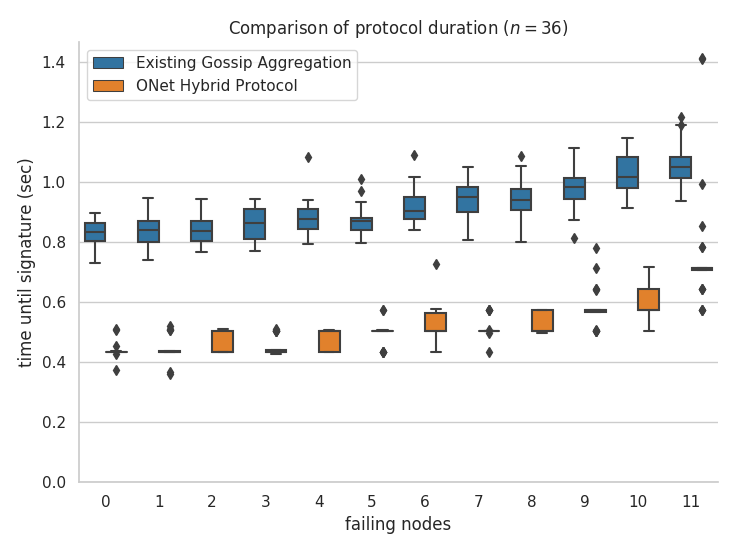
\includegraphics[width=0.91\textwidth]{images/round_wall_sum_36.png}
    \caption{Timings until a cosignature was returned using ONet Hybrid protocol vs Existing Gossip Aggregation.}
    \label{fig2time}
\end{figure}

\begin{figure}[H]
    \centering
    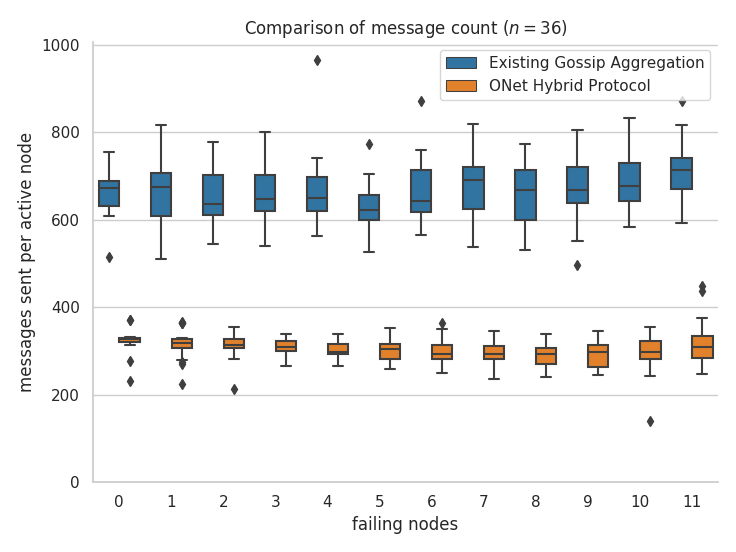
\includegraphics[width=0.91\textwidth]{images/bandwidth_msg_tx_sum_36.png}
    \caption{Number of messages sent per active node using ONet Hybrid protocol vs Existing Gossip Aggregation.}
    \label{fig2num}
\end{figure}

\begin{figure}[H]
    \centering
    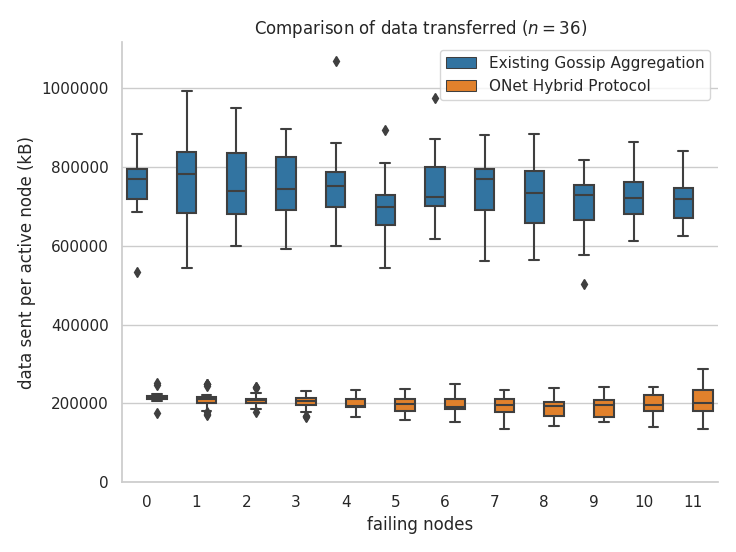
\includegraphics[width=0.91\textwidth]{images/bandwidth_tx_sum_36.png}
    \caption{Amounts of data transferred per active node using ONet Hybrid protocol vs Existing Gossip Aggregation.}
    \label{fig2data}
\end{figure}



\section{Conclusions}
Among the alternatative gossip-based aggregation implementations in the first part of the project, the new mask protocol is the best performing, since it keeps the same reasonably short time to produce a cosignature, doesn't have extreme outliers in the protocol duration. and while the number of messages exchanged is higher, the amount of data transferred is lower than the previous implementation.
Taking into account the gossip protocol model change from a push-only to a push and pull one, the performance improvements on these metrics are reasonable.
With the mask implementation we have also experimentally backed up the property of gossip protocol theory where it grows roughly like a function $O(log(n))$ of the number of nodes $n$.

For the mask aggregation protocol, the results are not good because of the mentioned constant propagation of all possible combinations of multi-signatures, which creates many unnecessary messages being sent around. The model had good intentions of trying to find the multi-signatures that can be aggregated to reach the threshold much faster by pulling these combinations, but this created not only an increase in the number of messages and bandwidth used, but also the duration of the protocol. This is because not only single signatures are being propagated, but also all possible multi-signature combinations are being passed around between nodes. In Figure~\ref{fig1time}, we can observe that with more nodes, the duration increases almost in an exponential way, which is not good at all.

For the second part of the project, the hybrid protocol implemented using ONet has a better performance than the existing gossip protocol, since it creates trees in the first part of a propagation round, and then gossips the message in the second part of it. This allows the new protocol to send less messages if the tree part of the propagation doesn't fail. If failure in an internal node causes it to block their children in the tree part, this problem will be overcome in the gossip part of the propagation.

The newly implemented protocols still have some limitations.
They do not adapt to the properties of the network, such as the network message delay, because ideally, a gossip protocol would send fewer messages per second in a slower network.
Due to the inherent randomness in the gossip protocol and the unpredictability of network message delays, there is no definite upper limit for the protocol duration.
Membership needs to be closed for the duration of the protocol, and all nodes need to know each other's identities and public keys beforehand.
For security against man-in-the-middle attacks, the protocol needs authenticated channels for messages.

There are some improvements that could be future work to expand the possible uses and improve the speed and efficiency of the protocols. The selection of peers who will receive a rumor in a gossiping round could be done in a different way than random picks. There is also the pending completion of the implementation of the protocol that uses homomorphic subtraction of signatures to use in a different aggregation. This would allow earlier aggregation and in theory this would reduce the bandwidth used. Finally, formal proof of all of the protocol's properties, and a more complete statistical analysis would be useful to make these implementations more attractive to applications that could potentially use them.
\newpage
\raggedright
\addcontentsline{toc}{section}{References}
\bibliographystyle{unsrt}
\bibliography{references}
\newpage



\appendix
\section{Appendix: Installing and running the program}
\label{axinstall}

The code for the program is published on GitHub~\cite{SemProjElias}.
It can be installed using Go~1.13 by running
\begin{verbatim}
go get github.com/dedis/student_19_elias
\end{verbatim}

Make sure that go.mod is pointing to the correct version of ONet. If needed, get the following ONet version (which has HybridRumor) and in go.mod point to the directory where this was cloned:
\begin{verbatim}
go get github.com/dedis/student_19_elias_onet
\end{verbatim}

Then navigate to the directory
\begin{verbatim}
student_elias/blscosi_hybrid_rumor/blscosi_hybrid_rumor/
\end{verbatim}
and running this command:
\begin{verbatim}
go install
\end{verbatim}

To launch a simulation, first install the simulation program in the directory
\begin{verbatim}
student_elias/blscosi_hybrid_rumor/simulation_bundle/
\end{verbatim}
again with the same command as above:
\begin{verbatim}
go install
\end{verbatim}
Then use a .toml file to set the parameters when running the command:
\begin{verbatim}
simulation_bundle local.toml
\end{verbatim}
\section{Appendix: Full results}
\label{axresults}

This appendix contains all the simulation results with the parameters mentioned in chapter 4.
The most important difference between graphs is the number of nodes in the simulation.
The y-axis starts at~0 in all graphs for better readability.
Results from Section~\ref{evares} are repeated here for the sake of completeness.


\subsection*{Comparison of the gossip protocol implementations }

\begin{figure}[H]
    \centering
    \begin{minipage}{0.5\textwidth}
        \centering
        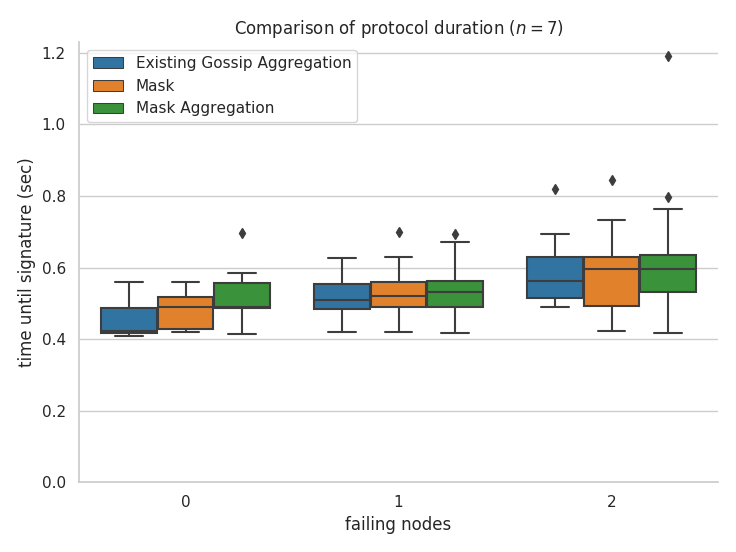
\includegraphics[width=\textwidth]{images/aggregation_round_wall_sum_7.png}
        \captionsetup{labelformat=empty}
        \caption{Protocol duration, $n = 7$}
    \end{minipage}\hfill
    \begin{minipage}{0.5\textwidth}
        \centering
        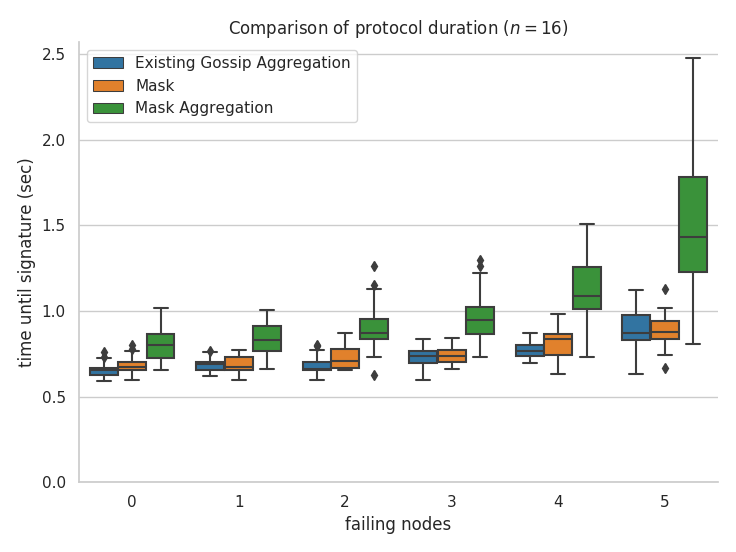
\includegraphics[width=\textwidth]{images/aggregation_round_wall_sum_16.png}
        \captionsetup{labelformat=empty}
        \caption{Protocol duration, $n = 16$}
    \end{minipage}\hfill
\end{figure}

\begin{figure}[H]
    \centering
    \begin{minipage}{0.5\textwidth}
        \centering
        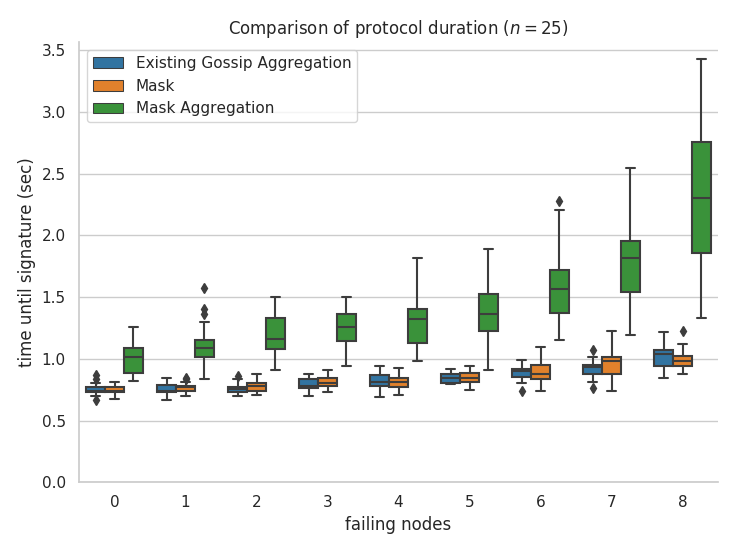
\includegraphics[width=\textwidth]{images/aggregation_round_wall_sum_25.png}
        \captionsetup{labelformat=empty}
        \caption{Protocol duration, $n = 25$}
    \end{minipage}\hfill
    \begin{minipage}{0.5\textwidth}
        \centering
        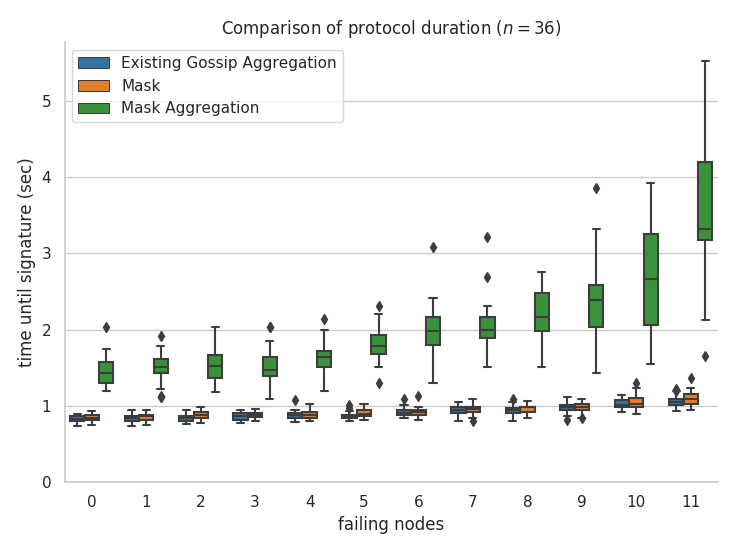
\includegraphics[width=\textwidth]{images/aggregation_round_wall_sum_36.png}
        \captionsetup{labelformat=empty}
        \caption{Protocol duration, $n = 36$}
    \end{minipage}\hfill
\end{figure}


\begin{figure}[H]
    \centering
    \begin{minipage}{0.5\textwidth}
        \centering
        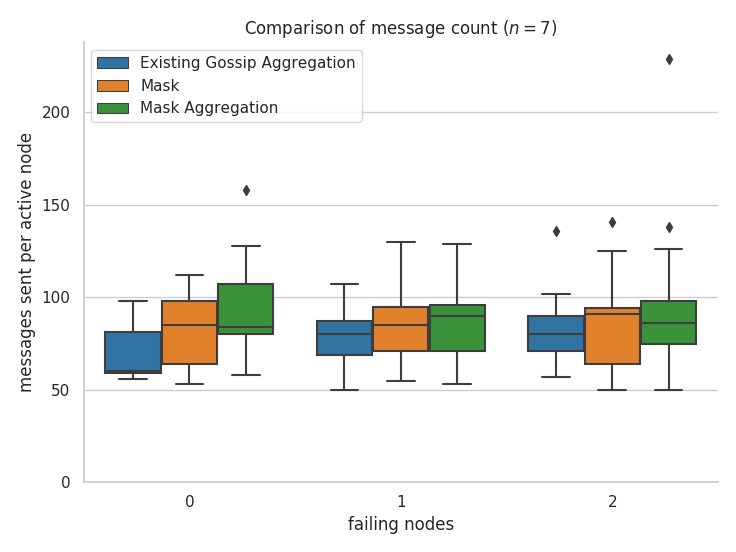
\includegraphics[width=\textwidth]{images/aggregation_bandwidth_msg_tx_sum_7.png}
        \captionsetup{labelformat=empty}
        \caption{Number of messages sent, $n = 7$}
    \end{minipage}\hfill
    \begin{minipage}{0.5\textwidth}
        \centering
        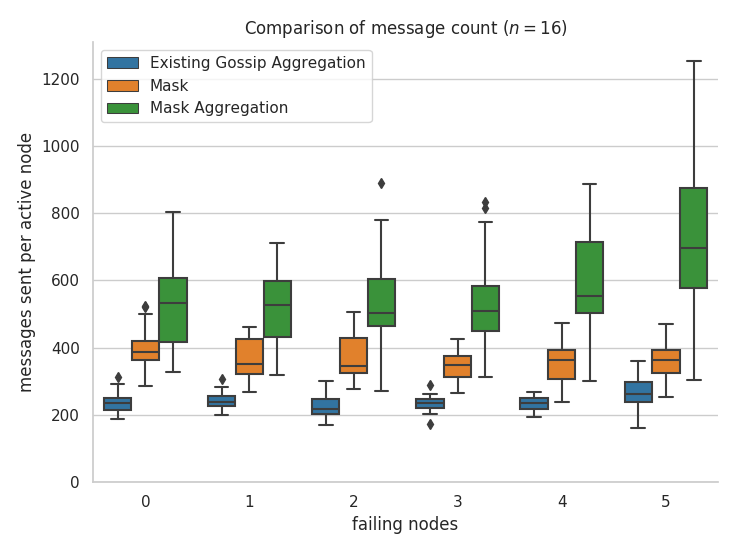
\includegraphics[width=\textwidth]{images/aggregation_bandwidth_msg_tx_sum_16.png}
        \captionsetup{labelformat=empty}
        \caption{Number of messages sent, $n = 16$}
    \end{minipage}\hfill
\end{figure}

\begin{figure}[H]
    \centering
    \begin{minipage}{0.5\textwidth}
        \centering
        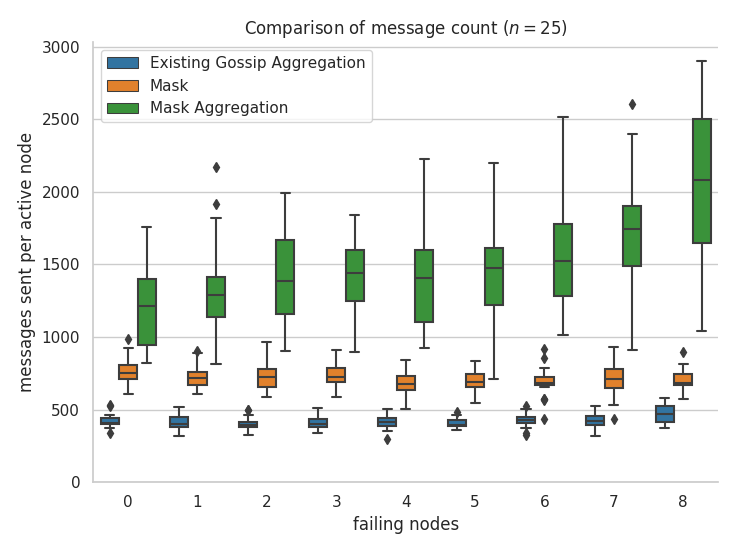
\includegraphics[width=\textwidth]{images/aggregation_bandwidth_msg_tx_sum_25.png}
        \captionsetup{labelformat=empty}
        \caption{Number of messages sent, $n = 25$}
    \end{minipage}\hfill
    \begin{minipage}{0.5\textwidth}
        \centering
        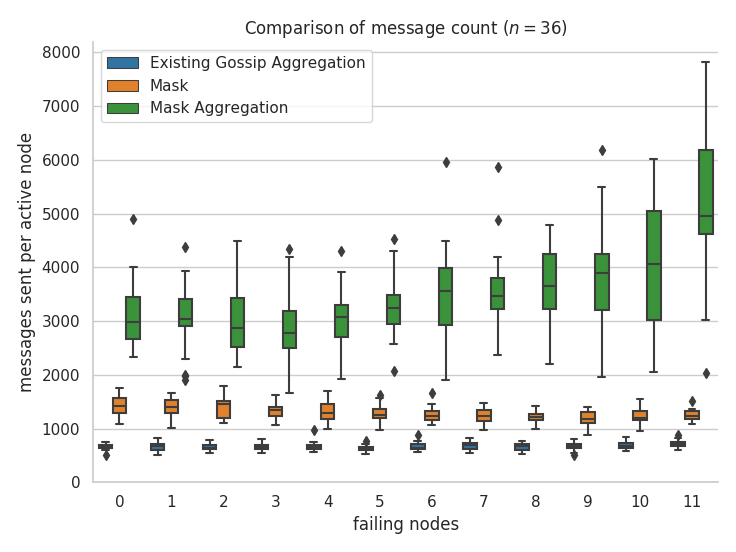
\includegraphics[width=\textwidth]{images/aggregation_bandwidth_msg_tx_sum_36.png}
        \captionsetup{labelformat=empty}
        \caption{Number of messages sent, $n = 36$}
    \end{minipage}\hfill
\end{figure}

\begin{figure}[H]
    \centering
    \begin{minipage}{0.5\textwidth}
        \centering
        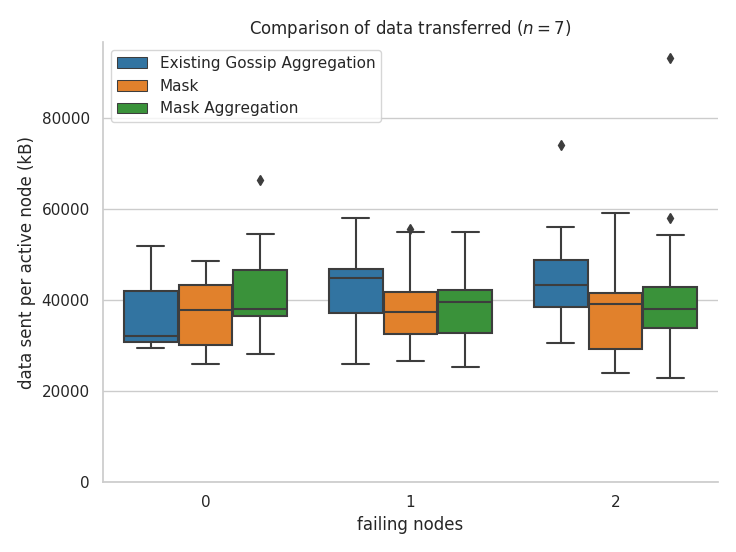
\includegraphics[width=\textwidth]{images/aggregation_bandwidth_tx_sum_7.png}
        \captionsetup{labelformat=empty}
        \caption{Data transferred per active, $n = 7$}
    \end{minipage}\hfill
    \begin{minipage}{0.5\textwidth}
        \centering
        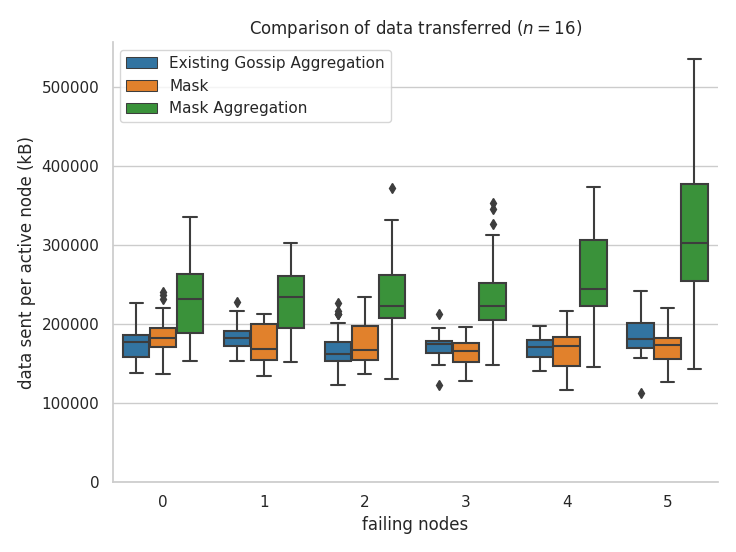
\includegraphics[width=\textwidth]{images/aggregation_bandwidth_tx_sum_16.png}
        \captionsetup{labelformat=empty}
        \caption{Data transferred per active, $n = 16$}
    \end{minipage}\hfill
\end{figure}

\begin{figure}[H]
    \centering
    \begin{minipage}{0.5\textwidth}
        \centering
        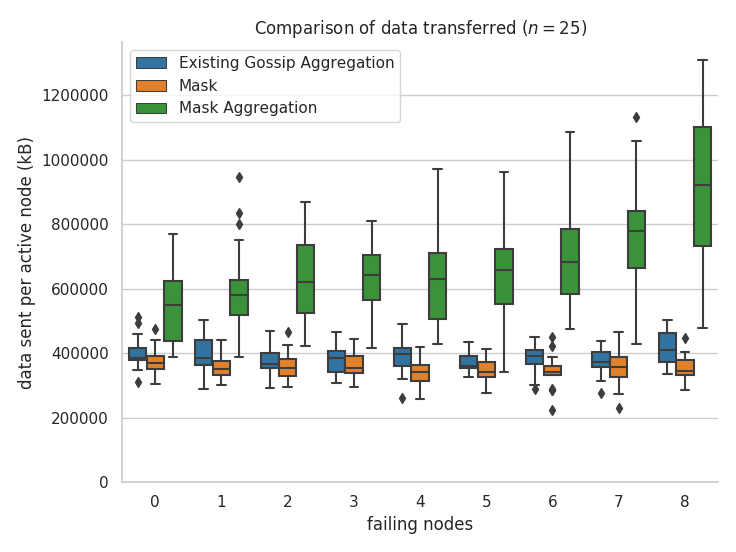
\includegraphics[width=\textwidth]{images/aggregation_bandwidth_tx_sum_25.png}
        \captionsetup{labelformat=empty}
        \caption{Data transferred per active, $n = 25$}
    \end{minipage}\hfill
    \begin{minipage}{0.5\textwidth}
        \centering
        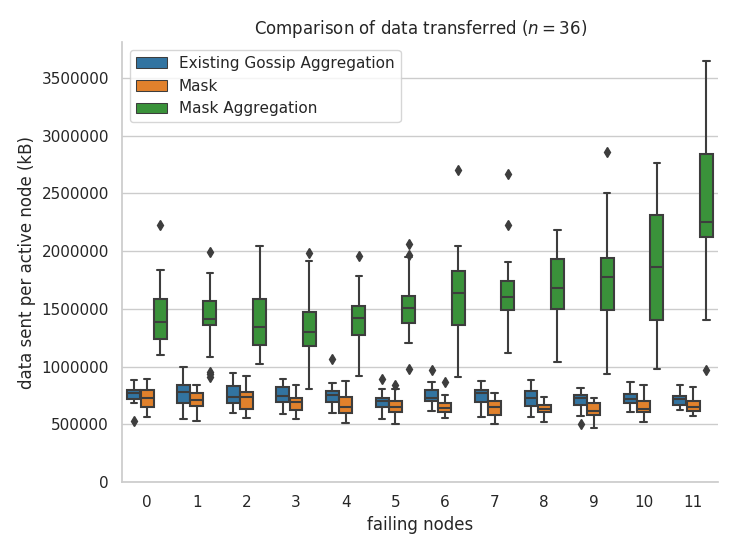
\includegraphics[width=\textwidth]{images/aggregation_bandwidth_tx_sum_36.png}
        \captionsetup{labelformat=empty}
        \caption{Data transferred per active, $n = 36$}
    \end{minipage}\hfill
\end{figure}

\subsection*{Comparison  of  the  ONet  implementation  with  the  existing Gossip aggregation}

\begin{figure}[H]
    \centering
    \begin{minipage}{0.5\textwidth}
        \centering
        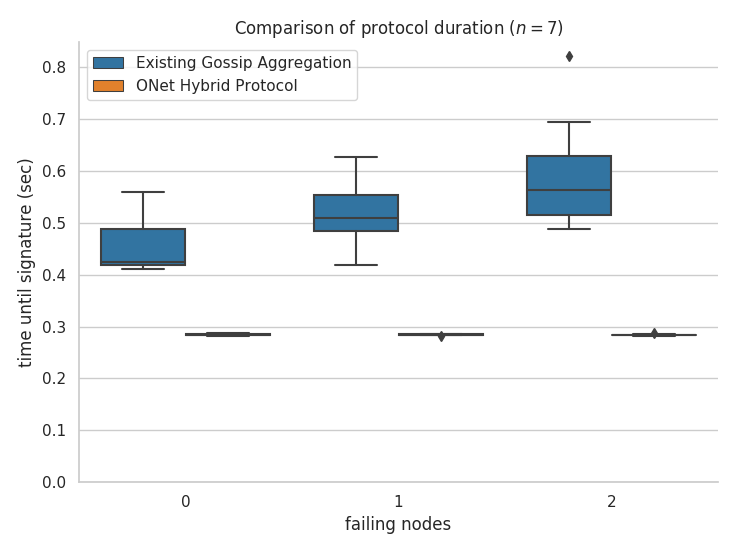
\includegraphics[width=\textwidth]{images/round_wall_sum_7.png}
        \captionsetup{labelformat=empty}
        \caption{Protocol duration, $n = 7$}
    \end{minipage}\hfill
    \begin{minipage}{0.5\textwidth}
        \centering
        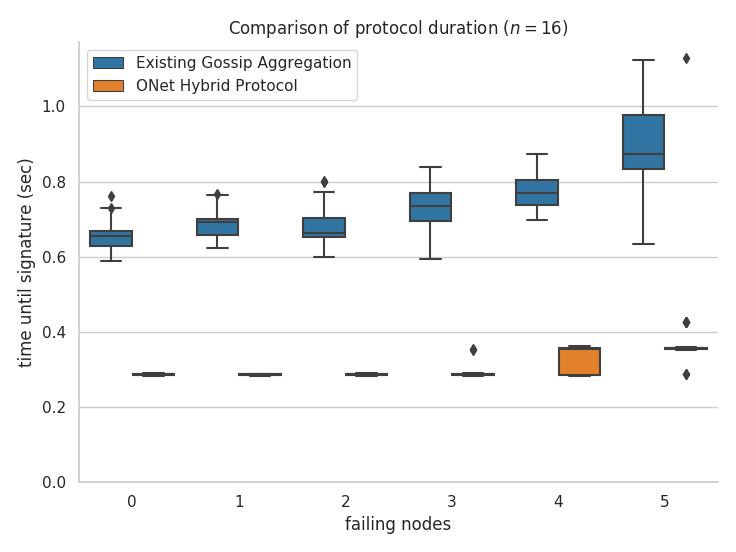
\includegraphics[width=\textwidth]{images/round_wall_sum_16.png}
        \captionsetup{labelformat=empty}
        \caption{Protocol duration, $n = 16$}
    \end{minipage}\hfill
\end{figure}

\begin{figure}[H]
    \centering
    \begin{minipage}{0.5\textwidth}
        \centering
        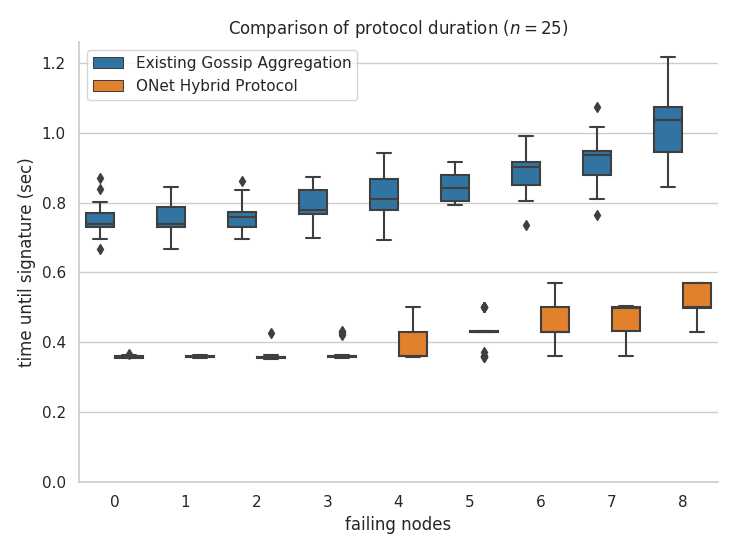
\includegraphics[width=\textwidth]{images/round_wall_sum_25.png}
        \captionsetup{labelformat=empty}
        \caption{Protocol duration, $n = 25$}
    \end{minipage}\hfill
    \begin{minipage}{0.5\textwidth}
        \centering
        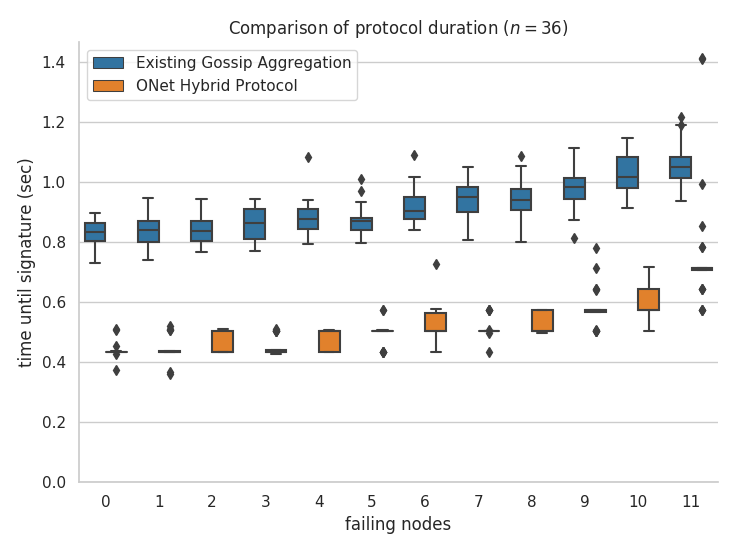
\includegraphics[width=\textwidth]{images/round_wall_sum_36.png}
        \captionsetup{labelformat=empty}
        \caption{Protocol duration, $n = 36$}
    \end{minipage}\hfill
\end{figure}


\begin{figure}[H]
    \centering
    \begin{minipage}{0.5\textwidth}
        \centering
        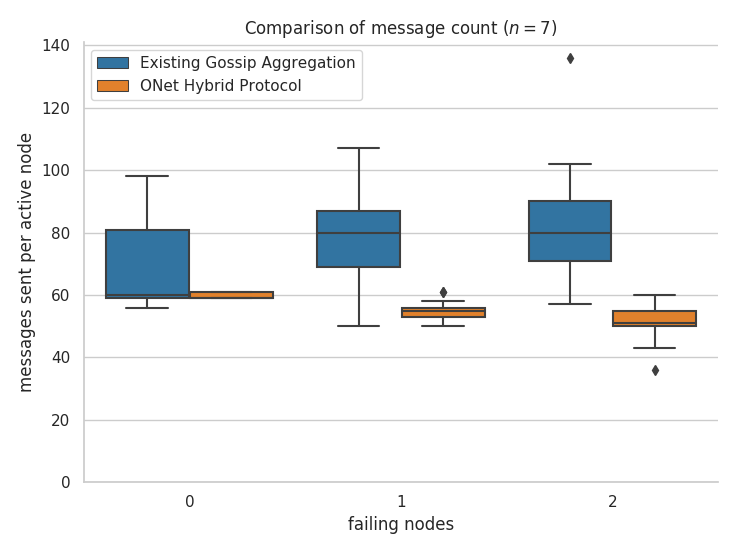
\includegraphics[width=\textwidth]{images/bandwidth_msg_tx_sum_7.png}
        \captionsetup{labelformat=empty}
        \caption{Number of messages sent, $n = 7$}
    \end{minipage}\hfill
    \begin{minipage}{0.5\textwidth}
        \centering
        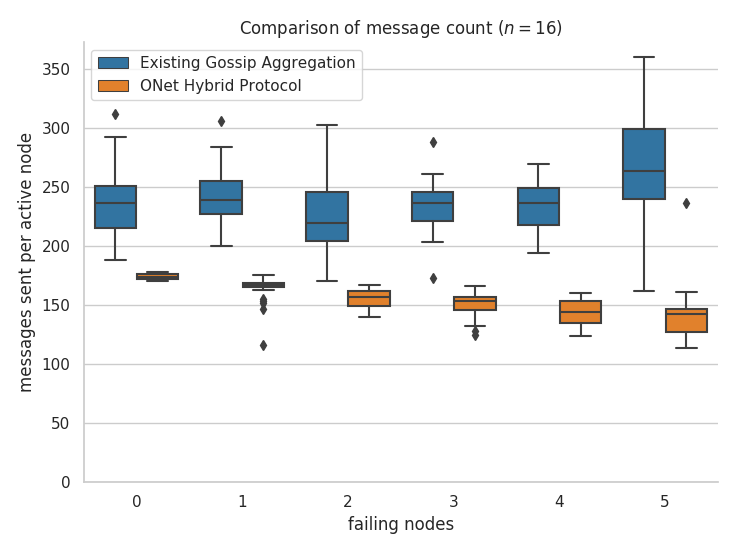
\includegraphics[width=\textwidth]{images/bandwidth_msg_tx_sum_16.png}
        \captionsetup{labelformat=empty}
        \caption{Number of messages sent, $n = 16$}
    \end{minipage}\hfill
\end{figure}

\begin{figure}[H]
    \centering
    \begin{minipage}{0.5\textwidth}
        \centering
        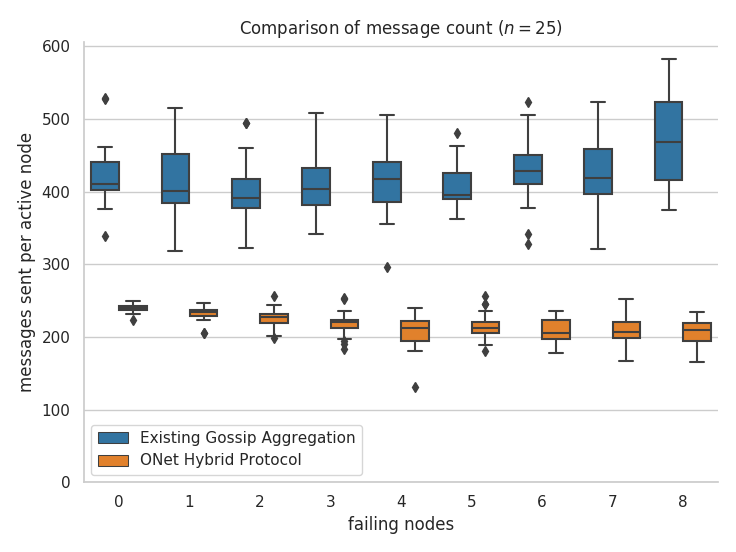
\includegraphics[width=\textwidth]{images/bandwidth_msg_tx_sum_25.png}
        \captionsetup{labelformat=empty}
        \caption{Number of messages sent, $n = 25$}
    \end{minipage}\hfill
    \begin{minipage}{0.5\textwidth}
        \centering
        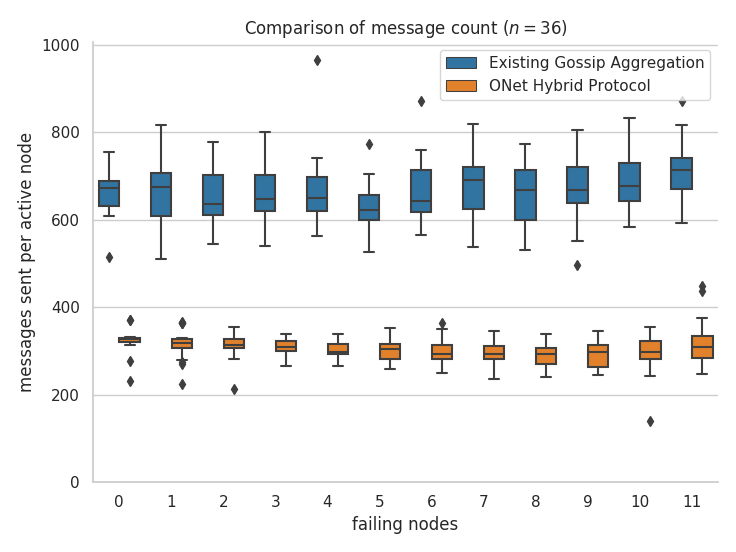
\includegraphics[width=\textwidth]{images/bandwidth_msg_tx_sum_36.png}
        \captionsetup{labelformat=empty}
        \caption{Number of messages sent, $n = 36$}
    \end{minipage}\hfill
\end{figure}

\begin{figure}[H]
    \centering
    \begin{minipage}{0.5\textwidth}
        \centering
        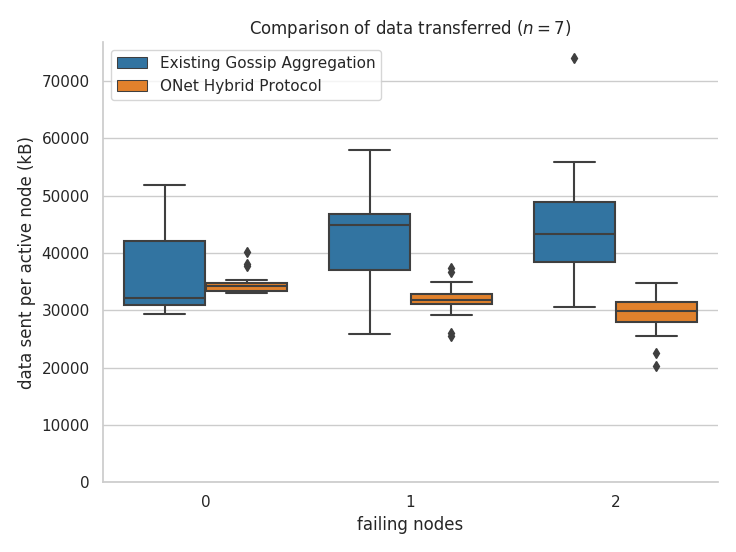
\includegraphics[width=\textwidth]{images/bandwidth_tx_sum_7.png}
        \captionsetup{labelformat=empty}
        \caption{Data transferred per active, $n = 7$}
    \end{minipage}\hfill
    \begin{minipage}{0.5\textwidth}
        \centering
        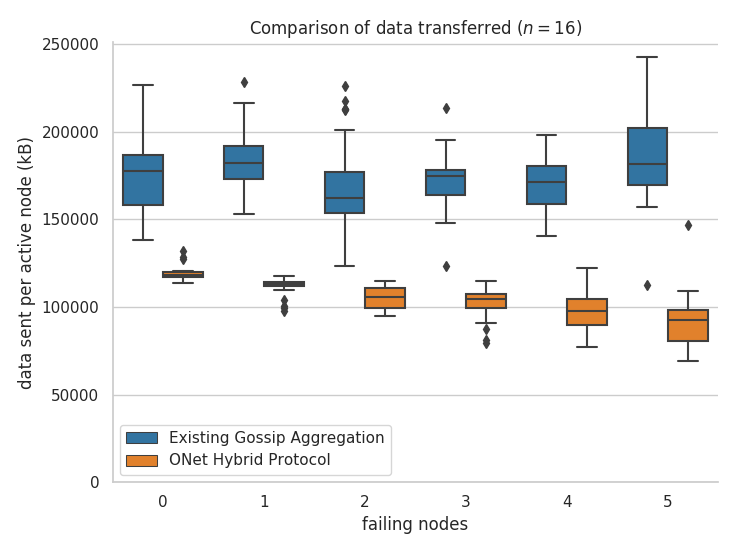
\includegraphics[width=\textwidth]{images/bandwidth_tx_sum_16.png}
        \captionsetup{labelformat=empty}
        \caption{Data transferred per active, $n = 16$}
    \end{minipage}\hfill
\end{figure}

\begin{figure}[H]
    \centering
    \begin{minipage}{0.5\textwidth}
        \centering
        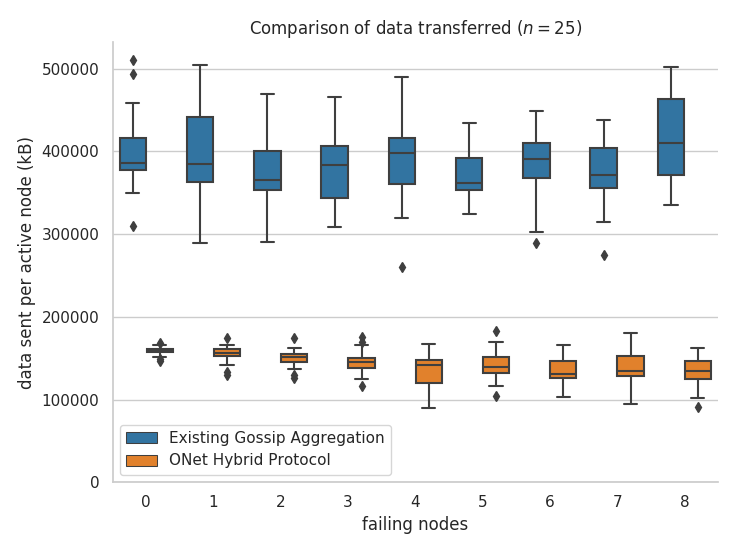
\includegraphics[width=\textwidth]{images/bandwidth_tx_sum_25.png}
        \captionsetup{labelformat=empty}
        \caption{Data transferred per active, $n = 25$}
    \end{minipage}\hfill
    \begin{minipage}{0.5\textwidth}
        \centering
        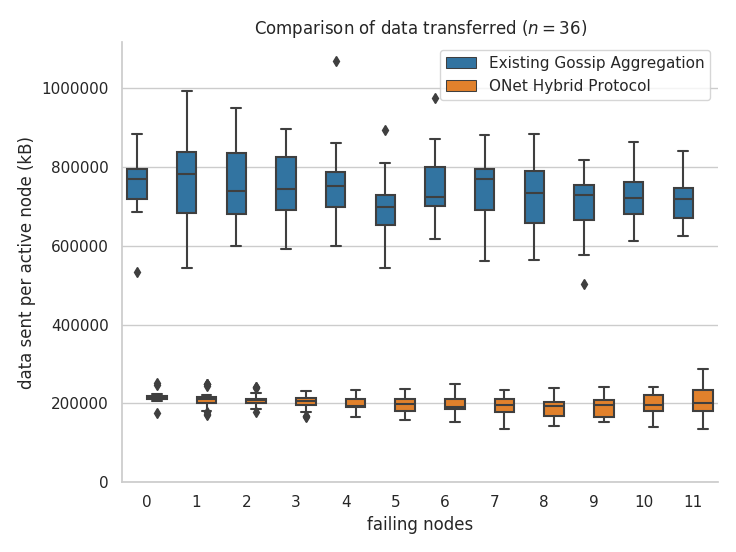
\includegraphics[width=\textwidth]{images/bandwidth_tx_sum_36.png}
        \captionsetup{labelformat=empty}
        \caption{Data transferred per active, $n = 36$}
    \end{minipage}\hfill
\end{figure}

\end{document}
